% THIS DOCUMENT IS FOLLOWS THE VOLERE TEMPLATE BY Suzanne Robertson and James Robertson
% ONLY THE SECTION HEADINGS ARE PROVIDED
%
% Initial draft from https://github.com/Dieblich/volere
%
% Risks are removed because they are covered by the Hazard Analysis
\documentclass[12pt]{article}
\usepackage{graphicx}
\usepackage{booktabs}
\usepackage{tabularx}
\usepackage{hyperref}
\usepackage{enumerate}
\hypersetup{
    bookmarks=true,         % show bookmarks bar?
      colorlinks=true,      % false: boxed links; true: colored links
    linkcolor=red,          % color of internal links (change box color with linkbordercolor)
    citecolor=green,        % color of links to bibliography
    filecolor=magenta,      % color of file links
    urlcolor=cyan           % color of external links
}

\newcommand{\lips}{\textit{Insert your content here.}}

%% Comments

\usepackage{color}

\newif\ifcomments\commentstrue %displays comments
%\newif\ifcomments\commentsfalse %so that comments do not display

\ifcomments
\newcommand{\authornote}[3]{\textcolor{#1}{[#3 ---#2]}}
\newcommand{\todo}[1]{\textcolor{red}{[TODO: #1]}}
\else
\newcommand{\authornote}[3]{}
\newcommand{\todo}[1]{}
\fi

\newcommand{\wss}[1]{\authornote{blue}{SS}{#1}} 
\newcommand{\plt}[1]{\authornote{magenta}{TPLT}{#1}} %For explanation of the template
\newcommand{\an}[1]{\authornote{cyan}{Author}{#1}}

%% Common Parts

\newcommand{\progname}{ProgName} % PUT YOUR PROGRAM NAME HERE
\newcommand{\authname}{Team \#, Team Name
\\ Student 1 name
\\ Student 2 name
\\ Student 3 name
\\ Student 4 name} % AUTHOR NAMES                  

\usepackage{hyperref}
    \hypersetup{colorlinks=true, linkcolor=blue, citecolor=blue, filecolor=blue,
                urlcolor=blue, unicode=false}
    \urlstyle{same}
                                


\begin{document}

\title{Software Requirements Specification for \progname: Document Management System} 
\author{\authname}
\date{\today}
	
\maketitle

~\newpage

\pagenumbering{roman}

\tableofcontents

~\newpage

\section*{Revision History}

\begin{tabularx}{\textwidth}{p{3cm}p{2cm}X}
\toprule {\textbf{Date}} & {\textbf{Version}} & {\textbf{Notes}}\\
\midrule
Date 1 & 1.0 & Notes\\
Date 2 & 1.1 & Notes\\
\bottomrule
\end{tabularx}

~\\

~\newpage
\section{Purpose of the Project}
\subsection{User Business}
\lips
\subsection{Goals of the Project}
\lips
\section{Stakeholders}
\subsection{Client}
\lips
\subsection{Customer}
\lips
\subsection{Other Stakeholders}
\lips
\subsection{Hands-On Users of the Project}
\lips
\subsection{Personas}
\lips
\subsection{Priorities Assigned to Users}
\lips
\subsection{User Participation}
\lips
\subsection{Maintenance Users and Service Technicians}
\lips

\section{Mandated Constraints}
\subsection{Solution Constraints}
\begin{enumerate} [{C-SOL}1.]
  \item System must be cloud-based to fit in with current existing systems at
  the City of Hamilton.
\end{enumerate}

\subsection{Implementation Environment of the Current System}
To understand the current practices at the City of Hamilton see the
\textit{Problem} section of the Problem Statement and Goals
\href{https://github.com/Spitgranger/capstone/blob/main/docs/ProblemStatementAndGoals/ProblemStatement.md#11-problem}
{here}.

\subsection{Partner or Collaborative Applications}
N/A
\subsection{Off-the-Shelf Software}
\begin{enumerate} [{C-OTS}1.]
  \item The system must integrate with Sharepoint to synchronize documents in
  Sharepoint with documents in the system.
  \item The system must integrate with Infor EAM, to show the status of work
  orders associated with a document.
  \item The system must integrate with MySDS to show relevent relevant SDS
  documents to users on a given site.
\end{enumerate}

\subsection{Anticipated Workplace Environment}
% TODO

\subsection{Schedule Constraints}
\begin{enumerate} [{C-SCH}1.]
  \item A requirement is to integrate with the Infor EAM system the city intends
  on using however, this system will not be available until February 2025, so no
  testing can be done on this system until then.

  \item The project deadline is April 2, 2025.
\end{enumerate}

\subsection{Budget Constraints}
\begin{enumerate} [{C-BDG}1.]
  \item Total expenses up until April 2, 2025 must not exceed \$750.
\end{enumerate}

\subsection{Enterprise Constraints}
N/A

\section{Naming Conventions and Terminology}
\subsection{Glossary of All Terms, Including Acronyms, Used by Stakeholders
involved in the Project}
\begin{itemize}
    \item BAS: Building Automation System.
    \item BCOS: Beyond Compliance Operating System.
    \item CMMS: Computerized Maintenance Management System.
    \item Confined Space: A partially or fully enclosed space, not designed for 
    continuous human occupancy, which has the potential for 
    atmospheric hazards.
    \item Controlled Space: A City defined space which has the potential to
    become a confined space.
    \item CSE: Confined Space Entry
    \item Dry Well: A room which houses industrial equipment such as pumps 
    and valves.
    \item Hazard Assessment Form: A form outlining potential
    hazards at a location.
    \item Hot Works: Work which produces ignition sources.
    Requires an accompanying hot works permit.
    \item HVAC: Heating, Ventilation, and Air Conditiong.
    \item Infor EAM: An Enterprise Asset Management system.
    \item PMATS: Plant Maintenance and Technical Services.
    \item PO: Purchase Order.
    \item PPE: Personal Protective Equipment.
    \item SCADA: Supervisory Control and Data Acquisition.
    \item SDS: Safety Data Sheets.
    \item Wet Well: A portion of a wastewater pumping station which receives
    and temporarily stores wastewater.
\end{itemize}

\section{Relevant Facts And Assumptions}
\subsection{Relevant Facts}
\begin{itemize}
    \item There are over 100 pumping stations throughout the City.
    \item There are dozens of service contracts, and many contractors
    and staff accessing stations each day.
    \item Some stations are in remote locations and may have poor cell signal.
    \item Some properties have multiple stations at the same site.
    \item Certain stations have special entry procedures.
\end{itemize}

\subsection{Business Rules}
\begin{itemize}
    \item External contractors do not have access to the internal network.
    \item Only authorized users can approve new procedures. 
    \item There is work at stations performed through a work order
    and routine work which doesn't have a work order.
    \item Employee collective agreements have restrictions on the release of
    GPS logs and video recording, which would require their approval.
\end{itemize}
\subsection{Assumptions}
\begin{itemize}
    \item Our project will focus on the application itself
    and our team will implement an authentication system adequate for our
    development. When the City integrates our application into their systems 
    they would replace our authentication system with one that meets their 
    detailed cybersecurity specifications.
    \item The existing entry and exit procedure for stations is not modified
    and our application will coexist with it.
\end{itemize}
\section{The Scope of the Work}
\subsection{The Current Situation}
The process currently employed by the stakeholder is predominantly a manual one.
Currently, contractor management is a time-consuming and manual effort. The 
following list identifies the current situation faced by the City:
\begin{itemize}
\item To distribute new or revised documentation to contractors, the City sends 
the documents manually through email. There are no automated processes in place
and this work flow is done manually for each document. There are dozens of
contractors which these documents need to be distributed to, and those
contractors themselves also change over time. The list of these contractors is
also managed manually.

\item Verification of work performed by contractors currently requires
a physical visit to site. There is no automated process to collect information 
such as photos of the work performed, other than manually through email.
\item It is currently difficult to know whether the labour cost
billed by the contractors on their invoices is reflective of the actual work
performed, as that information is only recorded in a physical logbook at each
site and is not electronic. A contractor could overcharge for the work and it
would be difficult to prove that their bill is inaccurate.

\end{itemize}

\subsection{The Context of the Work}
The below figure illustrates a high-level context model of the adjacent systems:
\begin{figure}[h]
\centering
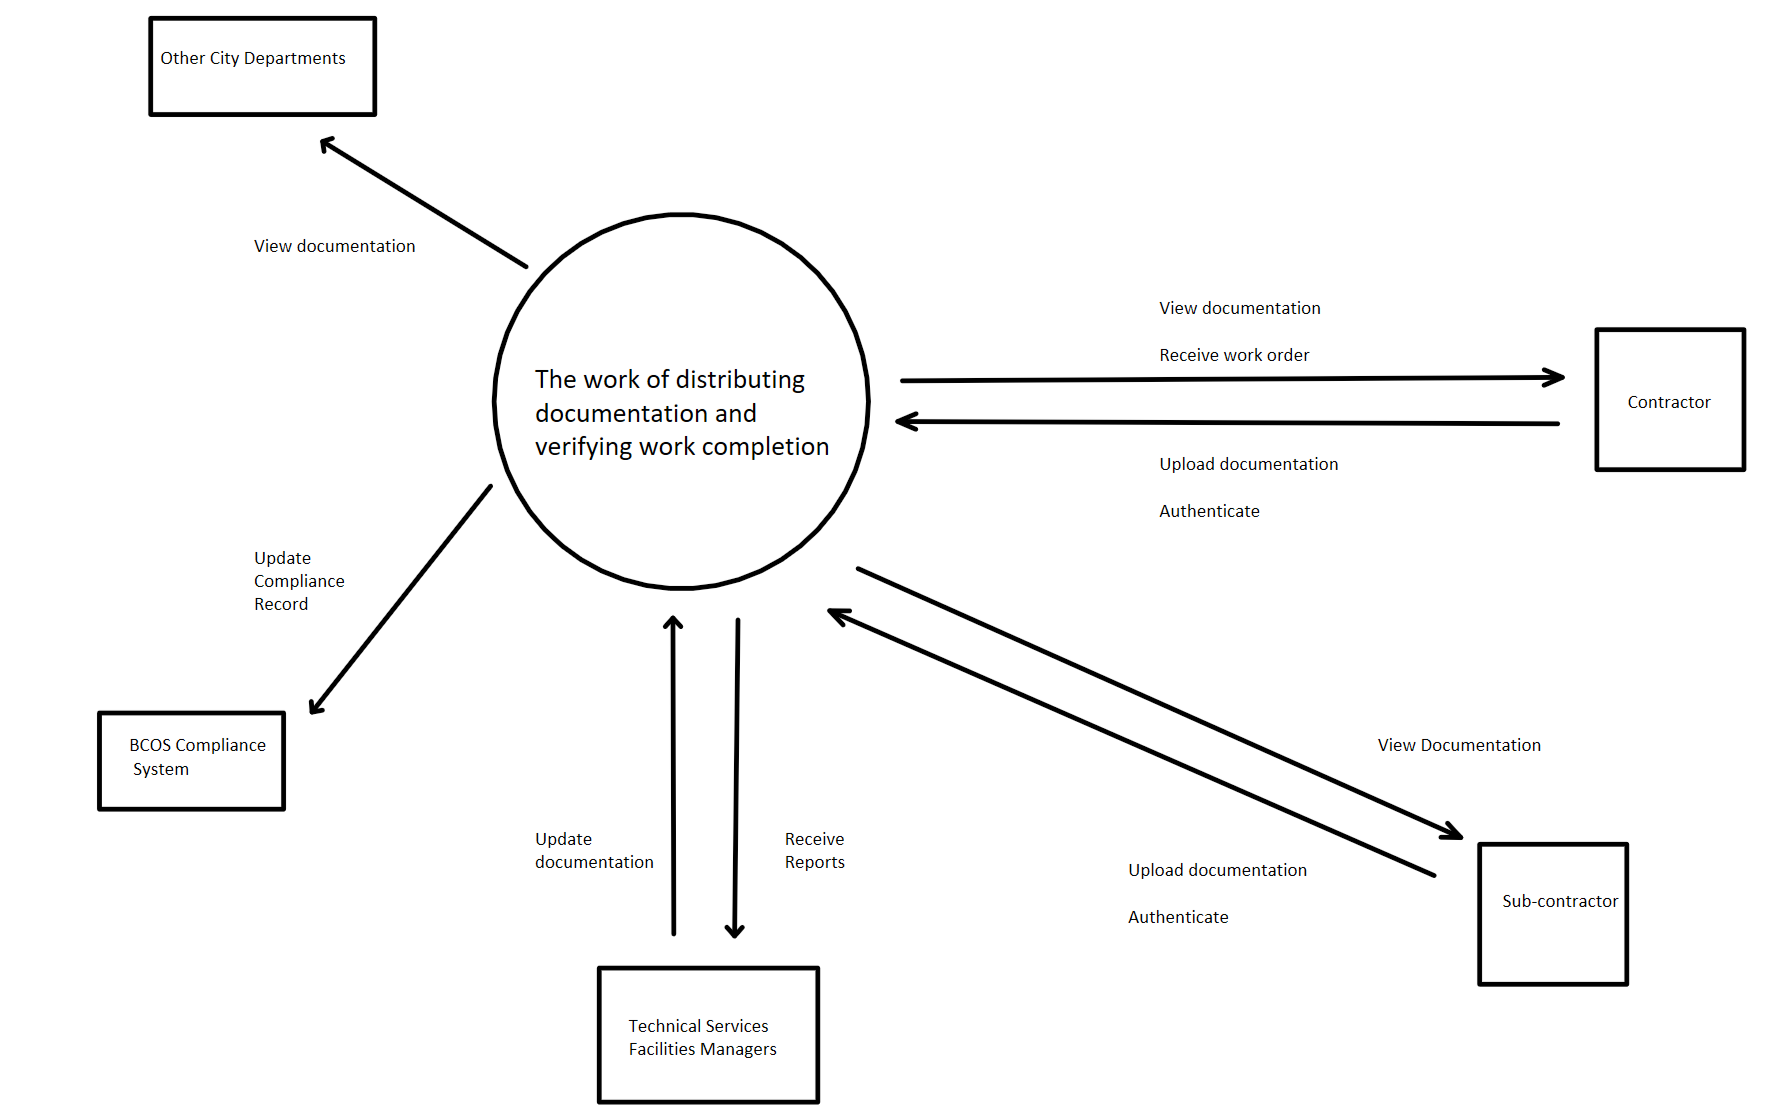
\includegraphics[width=1\textwidth]{4G06A-context-model.png}
\caption{Context model}
\end{figure}

\subsection{Work Partitioning}
\begin{tabular}{|l|l|}
\hline
\textbf{Event Name} & \textbf{Input and Output} \\
\hline
1. Contractor Login & Contractor email and one time password (in) \\
\hline
2. Contractor Authentication & GPS location (in) \\
\hline
3. Staff Login & Staff email and password (in) \\
\hline
4. Sign Document & unsigned document (in), signed document (out) \\
\hline
5. Upload Report & report file (in) \\
\hline
6. Export Reports & report specifications (in), report data (out)\\
\hline
7. View Station Entry Protocols & Station location (in), entry protocol (out)\\
\hline
8. Add Contractor to System & Contractor information (in) \\
\hline
9. View Contractor Summary & Contractor name (in), contractor data (out) \\
\hline
10. Certification Expiry & notice of document expiration to staff (out) \\
\hline
\end{tabular}

\subsection{Specifying a Business Use Case (BUC)}
The below points identify the business use cases for each of the
business events by number in section 6.3.\\

\begin{enumerate}
\item Contractor authenticates themselves to City systems, proving that they 
are authorized to be provided City information.\\
\item Contractor proves they are at a site for transparency when work is being 
completed.\\
\item Staff authenticates themselves as authorized to view private data.\\
\item Sign a document for contractual or regulatory purposes.\\
\item Documents are stored for record keeping and relevant stakeholders 
are notified as necessary.\\
\item Export data of a specific type specified by the user. For example, all 
crane inspections in the last year.\\
\item View a procedure of how staff and contractors must access a specified 
station.\\
\item New contractors are frequently onboarded, and their information is 
recorded by the facilities managers.\\
\item Facilities managers commonly need to see which employees of a contractor 
are due for their health and safety training, WSIB expiry, etc.\\
\item When a piece of documentation has expired, the next version needs to be 
put in place by staff to replace the expired version.\\
\end{enumerate}

\section{Business Data Model and Data Dictionary}
\subsection{Business Data Model}
\lips
\subsection{Data Dictionary}
\lips

\section{The Scope of the Product}
\subsection{Product Boundary}
\lips
\subsection{Product Use Case Table}
\lips
\subsection{Individual Product Use Cases (PUC's)}
\lips

\section{Functional Requirements}
\subsection{Functional Requirements}
\lips

\section{Look and Feel Requirements}
\subsection{Appearance Requirements}
\lips
\subsection{Style Requirements}
\lips

\section{Usability and Humanity Requirements}
\subsection{Ease of Use Requirements}
\begin{enumerate}[{UH-EU}1.]
    \item Users between the ages of {MIN\_AGE} and {MAX\_AGE},
      regardless of technical expertise, must be able to discover at least 70\% of
      the web application functionality within 10 minutes of being introduced to
      the system without any explaination or training.\\
      \textbf{Rationale}: Usability is of high importance to the users of the system.
      They will be mainly non-technical and must be able to learn and use the
      system quickly if it is to be of any value to them.
    \item The system should provide undo options or warnings for irreversible actions
      and 95\% of users should successfully use these features when prompted.\\
      \textbf{Rationale}: It is important to provide users of the systems with
      confirmations or warnings to prevent errors and if they do happen, make it
      easy to recover from them.
\end{enumerate}
\subsection{Personalization and Internationalization Requirements}
N/A
\subsection{Learning Requirements}
\begin{enumerate}[{UH-LR}1.]
    \item Users between the ages of {MIN\_AGE} and {MAX\_AGE} should not take
      more than 10 minutes to a learn feature of the web application after it is
      discovered.\\
      \textbf{Rationale}: A well designed system should give the user the most amount of
      functionality while being easy to understand. Users will be able to
      productive with the system in a short amount of time, reducing
      frustration.
    \item Users between the ages of {MIN\_AGE} and {MAX\_AGE} should be able to 
      complete the system onboarding tutorial or walkthrough within 5 minutes,
      and 80\% of users should report feeling confident in using the system afterward.\\
      \textbf{Rationale}: It is important that users are able to understand
      system documentation quickly to reduce mental overhead and increase
      productivity.
\end{enumerate}
\subsection{Understandability and Politeness Requirements}
\begin{enumerate}[{UH-UP}1.]
    \item The application must not contain symbols or allusions that
      may be offensive or politically charged.\\
      \textbf{Rationale}: As the system is to be used by people of diverse backgrounds
      and in a professional setting, it is important to keep a professional and
      neutural tone.
    \item System error messages should clearly explain the issue and suggest a resolution
      within 2 sentences. 90\% of users between the ages of {MIN\_AGE} and {MAX\_AGE}
      should report understanding the error and being able to resolve the issue without
      external support.\\
      \textbf{Rationale}: Useful system feedback is crucial since users need to
      know what the system is doing and how it interprets their input in order to
      determine next steps.
\end{enumerate}
\subsection{Accessibility Requirements}
TBD may be in constraints.
\section{Performance Requirements}
\subsection{Speed and Latency Requirements}
\lips
\subsection{Safety-Critical Requirements}
\lips
\subsection{Precision or Accuracy Requirements}
\lips
\subsection{Robustness or Fault-Tolerance Requirements}
\lips
\subsection{Capacity Requirements}
\lips
\subsection{Scalability or Extensibility Requirements}
\lips
\subsection{Longevity Requirements}
\lips

\section{Operational and Environmental Requirements}
\subsection{Expected Physical Environment}
\lips
\subsection{Wider Environment Requirements}
\lips
\subsection{Requirements for Interfacing with Adjacent Systems}
\lips
\subsection{Productization Requirements}
\lips
\subsection{Release Requirements}
\lips

\section{Maintainability and Support Requirements}
\subsection{Maintenance Requirements}
\begin{enumerate} [{MS-MTN}1.]
  \item A deployment of the system should take no more than 30 minutes (not
  including testing, and building time).
  \item The build time of the system should be no longer than 10 minutes (not
  including testing time).
  \item All automated tests should be able to run in under 10 minutes
  \item The system should have rigourous unit testing, line coverage should be
  $\ge$ 95\%, branch coverage should be $\ge$ 90\%.
  \item All core functionalities of the system (i.e. Functional Requirements),
  should have both automated end-to-end and unit testing corresponding to them
  \item The project must be able to be maintained by its users, as original
  developers will not be maintaining it after April 2, 2025.
\end{enumerate}
\subsection{Supportability Requirements}
\begin{enumerate} [{MS-SUP}1.]
  \item The application should have user-facing documentation on how to use the
  core functionalities of the system (i.e. functionalities described in
  functional requirements).
  \item The application should have documentation for all API's for future
  maintainers.
  \item The application should have documentation of internal functions and 
  abstractions for future maintainers.
  \item The application should have documentation on deployment, so users can
  deploy this application for themselves.
\end{enumerate}
\subsection{Adaptability Requirements}
\begin{enumerate} [{MS-ADP}1.]
  \item The application must be able to run on at least Google Chrome and
  Microsoft Edge browsers.
  \item The application must be able to run on tablets, smartphones, and
  laptops.
  \item The application must be able to run on Android, IOS, and Windows 10
\end{enumerate}

\section{Security Requirements}
\subsection{Access Requirements}
\lips
\subsection{Integrity Requirements}
\lips
\subsection{Privacy Requirements}
\lips
\subsection{Audit Requirements}
\lips
\subsection{Immunity Requirements}
\lips

\section{Cultural Requirements}
\subsection{Cultural Requirements}
\lips

\section{Compliance Requirements}
\subsection{Legal Requirements}
\lips
\subsection{Standards Compliance Requirements}
\lips

\section{Open Issues}
\lips

\section{Off-the-Shelf Solutions}
\subsection{Ready-Made Products}
Currently there exist many document management systems (i.e. Google Docs,
Sharepoint). However, They miss some of the clients major requirements. The
city wants to be able to integrate with their work order management system to
show the status of a work order that is associated with any given document,
but existing solutions do not provide this capability. They also want to be
able to verify that people were at a given site, when completing work, which
again there isn't a ready made product to do.
\subsection{Reusable Components}
We can use Sharepoint as file storage, since the city wants Sharepoint and this
system to be in sync, and storing the files in two seperate locations and then
syncing them will introduce a lot of overhead. Instead, all files can just be
stored on Sharepoint.
\subsection{Products That Can Be Copied}
N/A

\section{New Problems}
\subsection{Effects on the Current Environment}
\lips
\subsection{Effects on the Installed Systems}
\lips
\subsection{Potential User Problems}
\lips
\subsection{Limitations in the Anticipated Implementation Environment That May
Inhibit the New Product}
\lips
\subsection{Follow-Up Problems}
\lips

\section{Tasks}
\subsection{Project Planning}
\lips
\subsection{Planning of the Development Phases}
\lips

\section{Migration to the New Product}
\subsection{Requirements for Migration to the New Product}
\begin{enumerate} [{MI-NP}1.]
  \item The system must be compatible with existing user roles in Active
    Directory.\\
    \textbf{Rationale}: Compatibility with existing business rules is needed
    to ensure migration can be completed in a short period of time without
    having to defined new roles.
\end{enumerate}

\subsection{Data That Has to be Modified or Translated for the New System}
\begin{enumerate} [{MI-TR}1.]
  \item Information stored on paper must be digitized for consumption for the
    system.\\
    \textbf{Rationale}: Some content that the system is to consume has not yet
    been digitized. It will have to be digitized before the system is able to
    use it.
\end{enumerate}

\section{Costs}
\lips
\section{User Documentation and Training}
\subsection{User Documentation Requirements}
\lips
\subsection{Training Requirements}
\lips

\section{Waiting Room}
\lips

\section{Ideas for Solution}
\lips

\newpage{}
\section*{Appendix --- Reflection}
\subsection{Symbolic Parameters}
$\hypertarget{min_age}{MIN\_AGE}$ = 18\\
$\hypertarget{min_age}{MAX\_AGE}$ = 70\\

The information in this section will be used to evaluate the team members on the
graduate attribute of Lifelong Learning.  Please answer the following questions:

\begin{enumerate}
  \item What knowledge and skills will the team collectively need to acquire to
  successfully complete this capstone project?  Examples of possible knowledge
  to acquire include domain specific knowledge from the domain of your
  application, or software engineering knowledge, mechatronics knowledge or
  computer science knowledge.  Skills may be related to technology, or writing,
  or presentation, or team management, etc.  You should look to identify at
  least one item for each team member.
  \item For each of the knowledge areas and skills identified in the previous
  question, what are at least two approaches to acquiring the knowledge or
  mastering the skill?  Of the identified approaches, which will each team
  member pursue, and why did they make this choice?
\end{enumerate}

\end{document}
